%%%%%%%%%%%%%%%%%%%%%%%%%%%%%%%%%%%%%%%%%
% Short Sectioned Assignment
% LaTeX Template
% Version 1.0 (5/5/12)
%
% This template has been downloaded from:
% http://www.LaTeXTemplates.com
%
% Original author:
% Frits Wenneker (http://www.howtotex.com)
%
% License:
% CC BY-NC-SA 3.0 (http://creativecommons.org/licenses/by-nc-sa/3.0/)
%
%%%%%%%%%%%%%%%%%%%%%%%%%%%%%%%%%%%%%%%%%

%----------------------------------------------------------------------------------------
%	PACKAGES AND OTHER DOCUMENT CONFIGURATIONS
%----------------------------------------------------------------------------------------

\documentclass[titlepage, paper=a4, fontsize=11pt]{scrartcl} % A4 paper and 11pt font size

\usepackage[T1]{fontenc} % Use 8-bit encoding that has 256 glyphs
\usepackage{fourier} % Use the Adobe Utopia font for the document - comment this line to return to the LaTeX default
\usepackage[english]{babel} % English language/hyphenation
\usepackage{amsmath,amsfonts,amsthm} % Math packages
\usepackage{listings}

\usepackage{lipsum} % Used for inserting dummy 'Lorem ipsum' text into the template
\usepackage{graphicx}


\usepackage{sectsty} % Allows customizing section commands
\allsectionsfont{\centering \normalfont\scshape} % Make all sections centered, the default font and small caps

\usepackage{fancyhdr} % Custom headers and footers
\pagestyle{fancyplain} % Makes all pages in the document conform to the custom headers and footers
\fancyhead{} % No page header - if you want one, create it in the same way as the footers below
\fancyfoot[L]{} % Empty left footer
\fancyfoot[C]{} % Empty center footer
\fancyfoot[R]{\thepage} % Page numbering for right footer
\renewcommand{\headrulewidth}{0pt} % Remove header underlines
\renewcommand{\footrulewidth}{0pt} % Remove footer underlines
\setlength{\headheight}{13.6pt} % Customize the height of the header

\numberwithin{equation}{section} % Number equations within sections (i.e. 1.1, 1.2, 2.1, 2.2 instead of 1, 2, 3, 4)
\numberwithin{table}{section} % Number tables within sections (i.e. 1.1, 1.2, 2.1, 2.2 instead of 1, 2, 3, 4)

\setlength\parindent{0pt} % Removes all indentation from paragraphs - comment this line for an assignment with lots of text

%----------------------------------------------------------------------------------------
%	TITLE SECTION
%----------------------------------------------------------------------------------------

\newcommand{\horrule}[1]{\rule{\linewidth}{#1}} % Create horizontal rule command with 1 argument of height

\title{	
\normalfont \normalsize 
\textsc{University of Virginia} \\ [25pt] % Your university, school and/or department name(s)
\horrule{0.5pt} \\[0.4cm] % Thin top horizontal rule
\huge ECE/CS 5565 Homework 4 \\ % The assignment title
\horrule{2pt} \\[0.5cm] % Thick bottom horizontal rule
}

\author{Shawn (Shuoshuo) Chen\\sc7cq@virginia.edu} % Your name

\date{\normalsize\today} % Today's date or a custom date

\begin{document}

\maketitle % Print the title

%----------------------------------------------------------------------------------------
%	PROBLEM 27
%----------------------------------------------------------------------------------------

\section*{Problem 27}
\textbf{(a).}
Sequence number is $127+80=207$, source port is 302, destination port is 80. \\

\textbf{(b).}
The ACK number should be the next expected byte, which is the cumulative bytes plus one.
So the ACK number is 207, source port is 80 and destination port is 302. \\

\textbf{(c).}
The receiver is expecting the segment with seqnum=127, but it gets a segment with seqnum=207.
Then the receiver knows there is a missing segment. Accroding to the behavior of TCP. the receiver
would still ACK 127. \\

\textbf{(d).}
See figure \ref{fig:p27}.
\begin{figure}[!ht]
    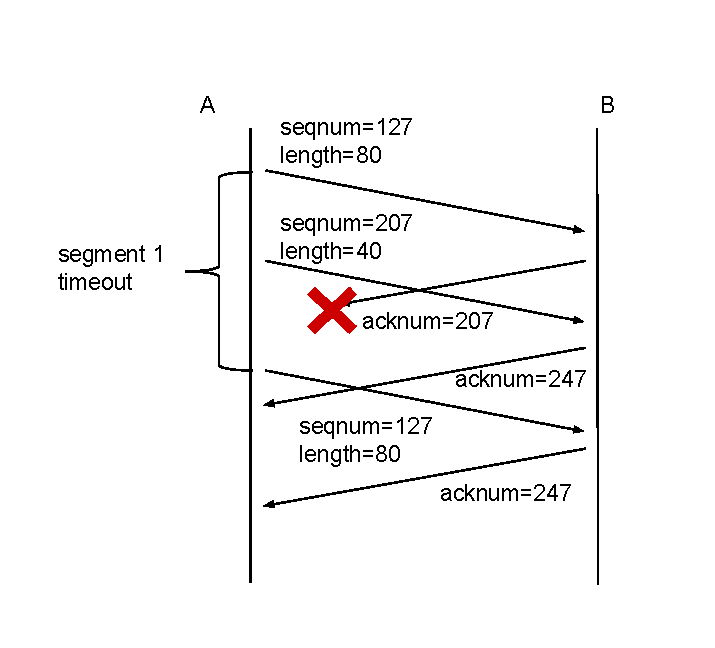
\includegraphics[width=\textwidth]{images/p27.pdf}
    \caption{Coomunication sequence between A and B}
    \label{fig:p27}
\end{figure}
\\


%----------------------------------------------------------------------------------------
%	PROBLEM 6
%----------------------------------------------------------------------------------------

\section*{Problem 6}
If the sender sends a packet with sequence number 1, and receiver confirms with an ACK 1.
But the ACK is corrupted when it reaches the sender. The sender then resends packet 1. However,
according to the FSM, receiver has already been waiting for packet 0. As a consequence, it rejects
the resent packet 1 with NAK back to the sender. The sender keeps sending packet 1 and the receiver
keeps rejecting. Both sides go into a deadlock state.
\\


%----------------------------------------------------------------------------------------
%	PROBLEM 8
%----------------------------------------------------------------------------------------
\section*{Problem 8}
Please see Figure \ref{fig:rdt3}.
\begin{figure}[!ht]
    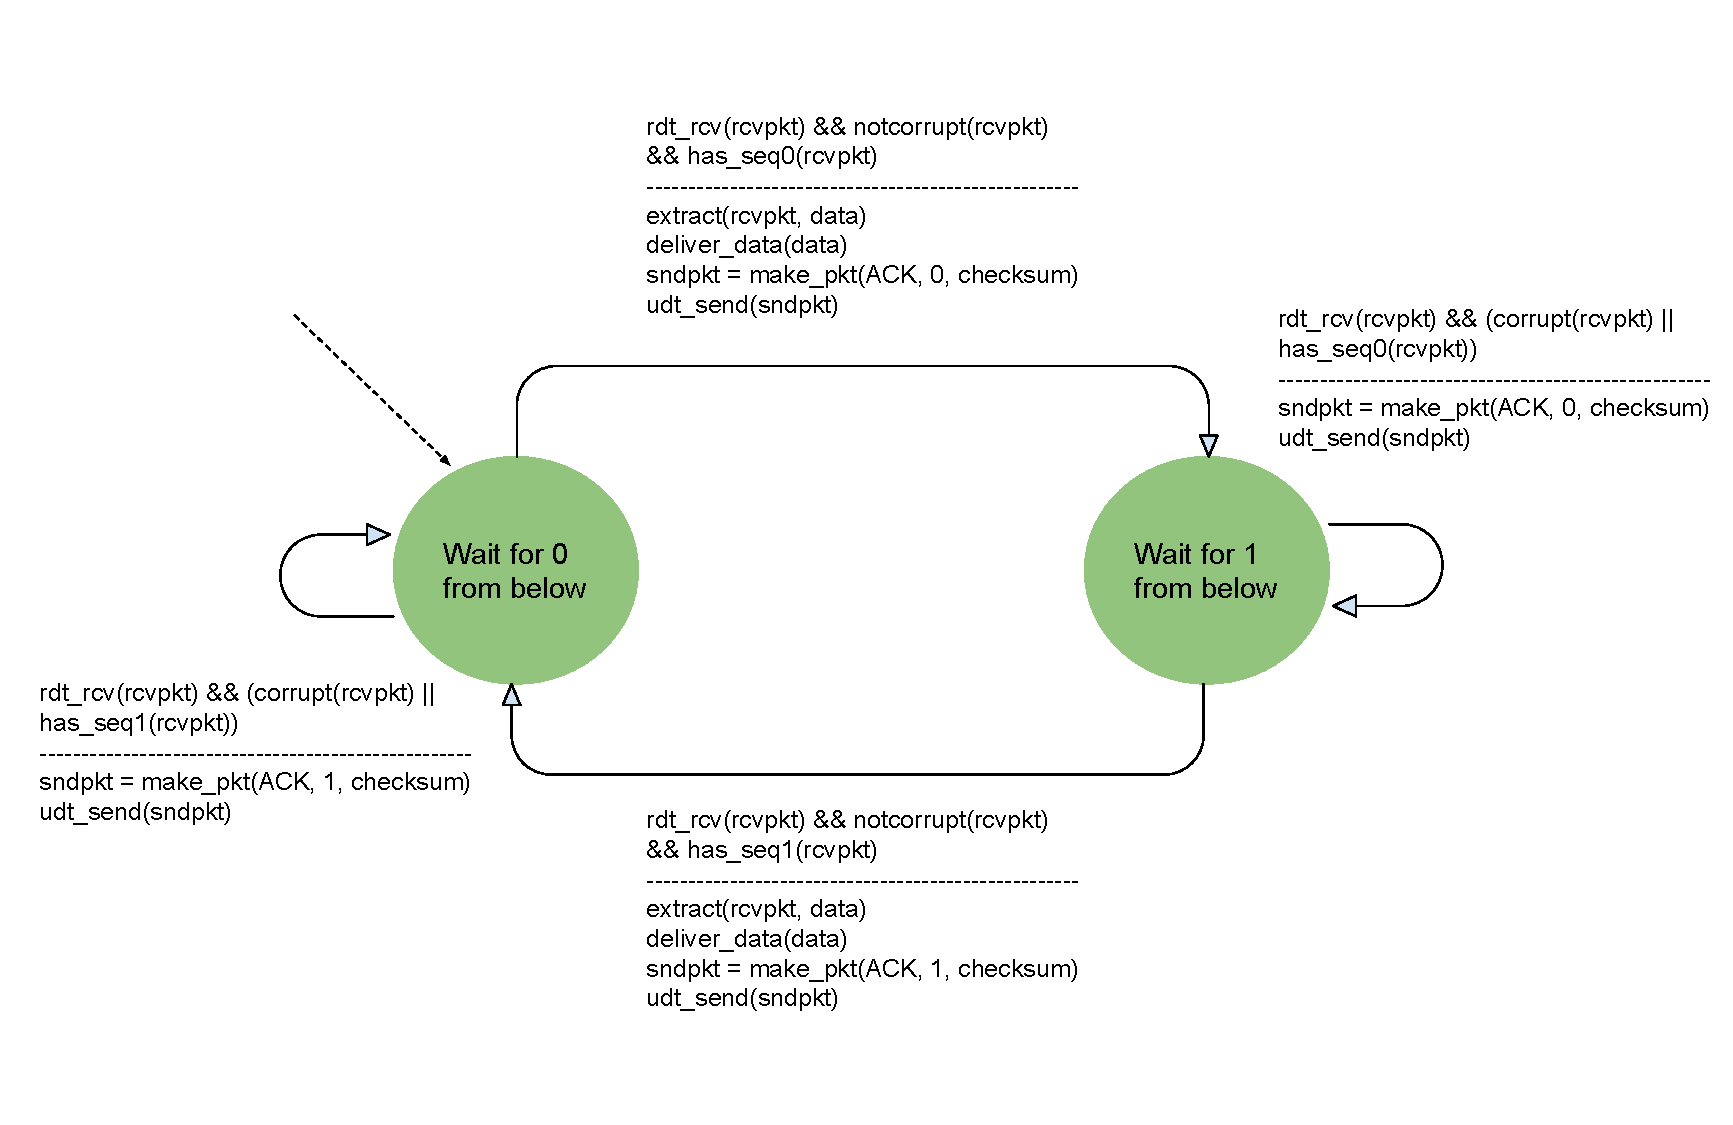
\includegraphics[width=\textwidth]{images/rdt3-rcv-FSM.pdf}
    \caption{Receiver FSM for rdt3.0}
    \label{fig:rdt3}
\end{figure}



%----------------------------------------------------------------------------------------
%	PROBLEM 11
%----------------------------------------------------------------------------------------

\section*{Problem 11}
If the receiver does not send back an ACK and the packet is corrupted, the sender will keep waiting until eventually an ACK shows up.
However, this is impossible to happen. And the receiver also keeps waiting until sender sends something
new. Thus, both the sender and receiver will enter a deadlock state. \\

Similarly, if there is no Wait-for-0-from-below self transition, same thing would happen and both sender
and receiver will enter a deadlock state.
\\

\newpage

%----------------------------------------------------------------------------------------
%	PROBLEM 12
%----------------------------------------------------------------------------------------

\section*{Problem 12}
The protocol will still work, but it would probably cause a huge amount of retransmission. \\
Imagine the timer is premature, thus it goes off before the first ACK comes back. An extra copy of
the packet is sent. Then if bit error occurs causing the ACK to be corrupted, another extra copy of the packet will be sent again. So in the worst case, a packet could be sent 3 times plus as many times as the number of ACKs for previous packets on the way.
\\


%----------------------------------------------------------------------------------------
%	PROBLEM 13
%----------------------------------------------------------------------------------------

\section*{Problem 13}
As figure \ref{fig:p13} shows, the first D0 is reordered and appears right before the new D0.
This would confuse the receiver since receiver might take the reordered D0, which it has already received,
as the new D0 expected.
\begin{figure}[!ht]
    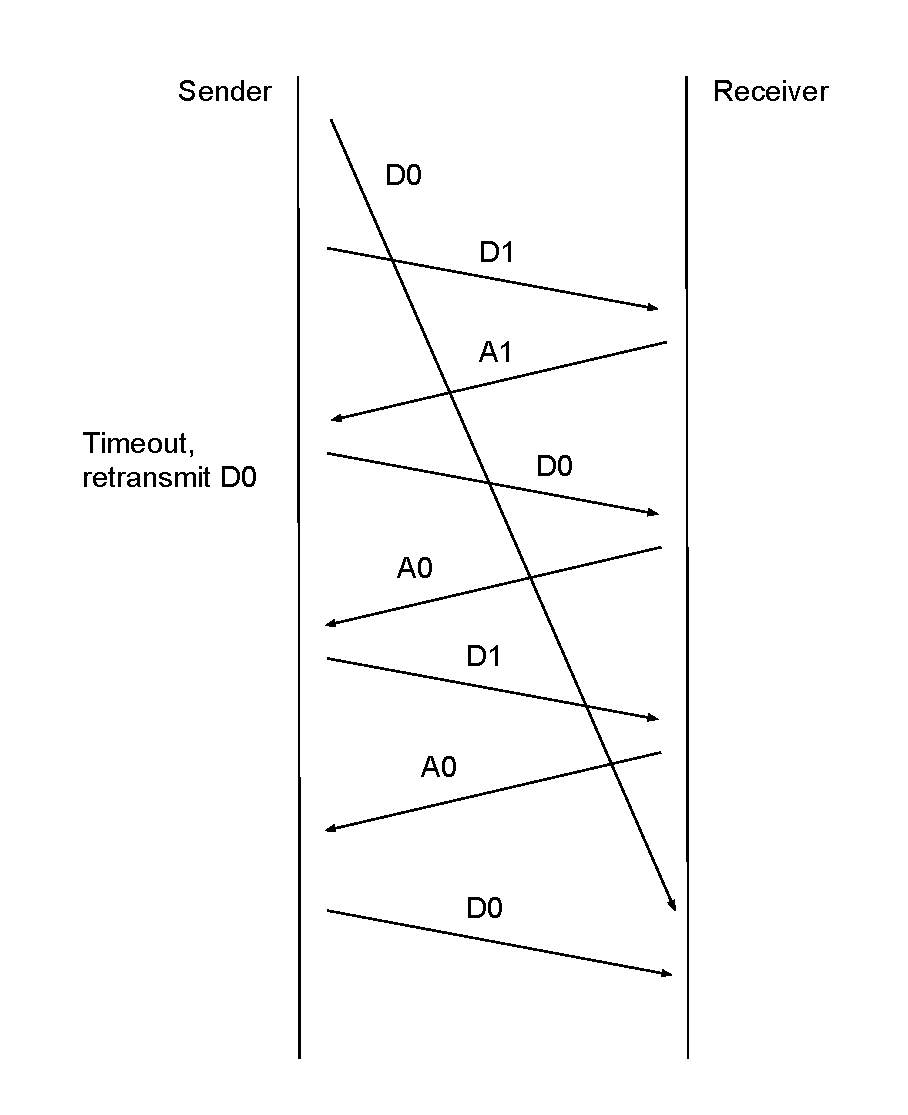
\includegraphics[width=\textwidth]{images/P13.pdf}
    \caption{Out-of-sequence problem}
    \label{fig:p13}
\end{figure}
\\


%----------------------------------------------------------------------------------------
%	PROBLEM 15
%----------------------------------------------------------------------------------------

\section*{Problem 15}
This is a pipelining scenario. According to the definition of utilization, there is:
\begin{align*} 
\begin{split}
U_{sender} = \frac{n*L/R}{RTT+L/R} \geq 0.98
\end{split}					
\end{align*}
where L = 1500 bytes, R = 1 Gbps, RTT = 0.03 sec and n is the window size.
Thus:
\begin{align*} 
\begin{split}
U_{sender} &= \frac{n*L/R}{RTT+L/R} \\
&=  \frac{n*1500*8/1000000000}{0.03+1500*8/1000000000} \geq 0.98
\end{split}					
\end{align*}
Solve for n, there is $n=2451$ packets.
\\


%----------------------------------------------------------------------------------------
%	PROBLEM 18
%----------------------------------------------------------------------------------------

\section*{Problem 18}
The FSM of this protocol is described by figure \ref{fig:p18-s} and figure \ref{fig:p18-r}.
\begin{figure}[!ht]
    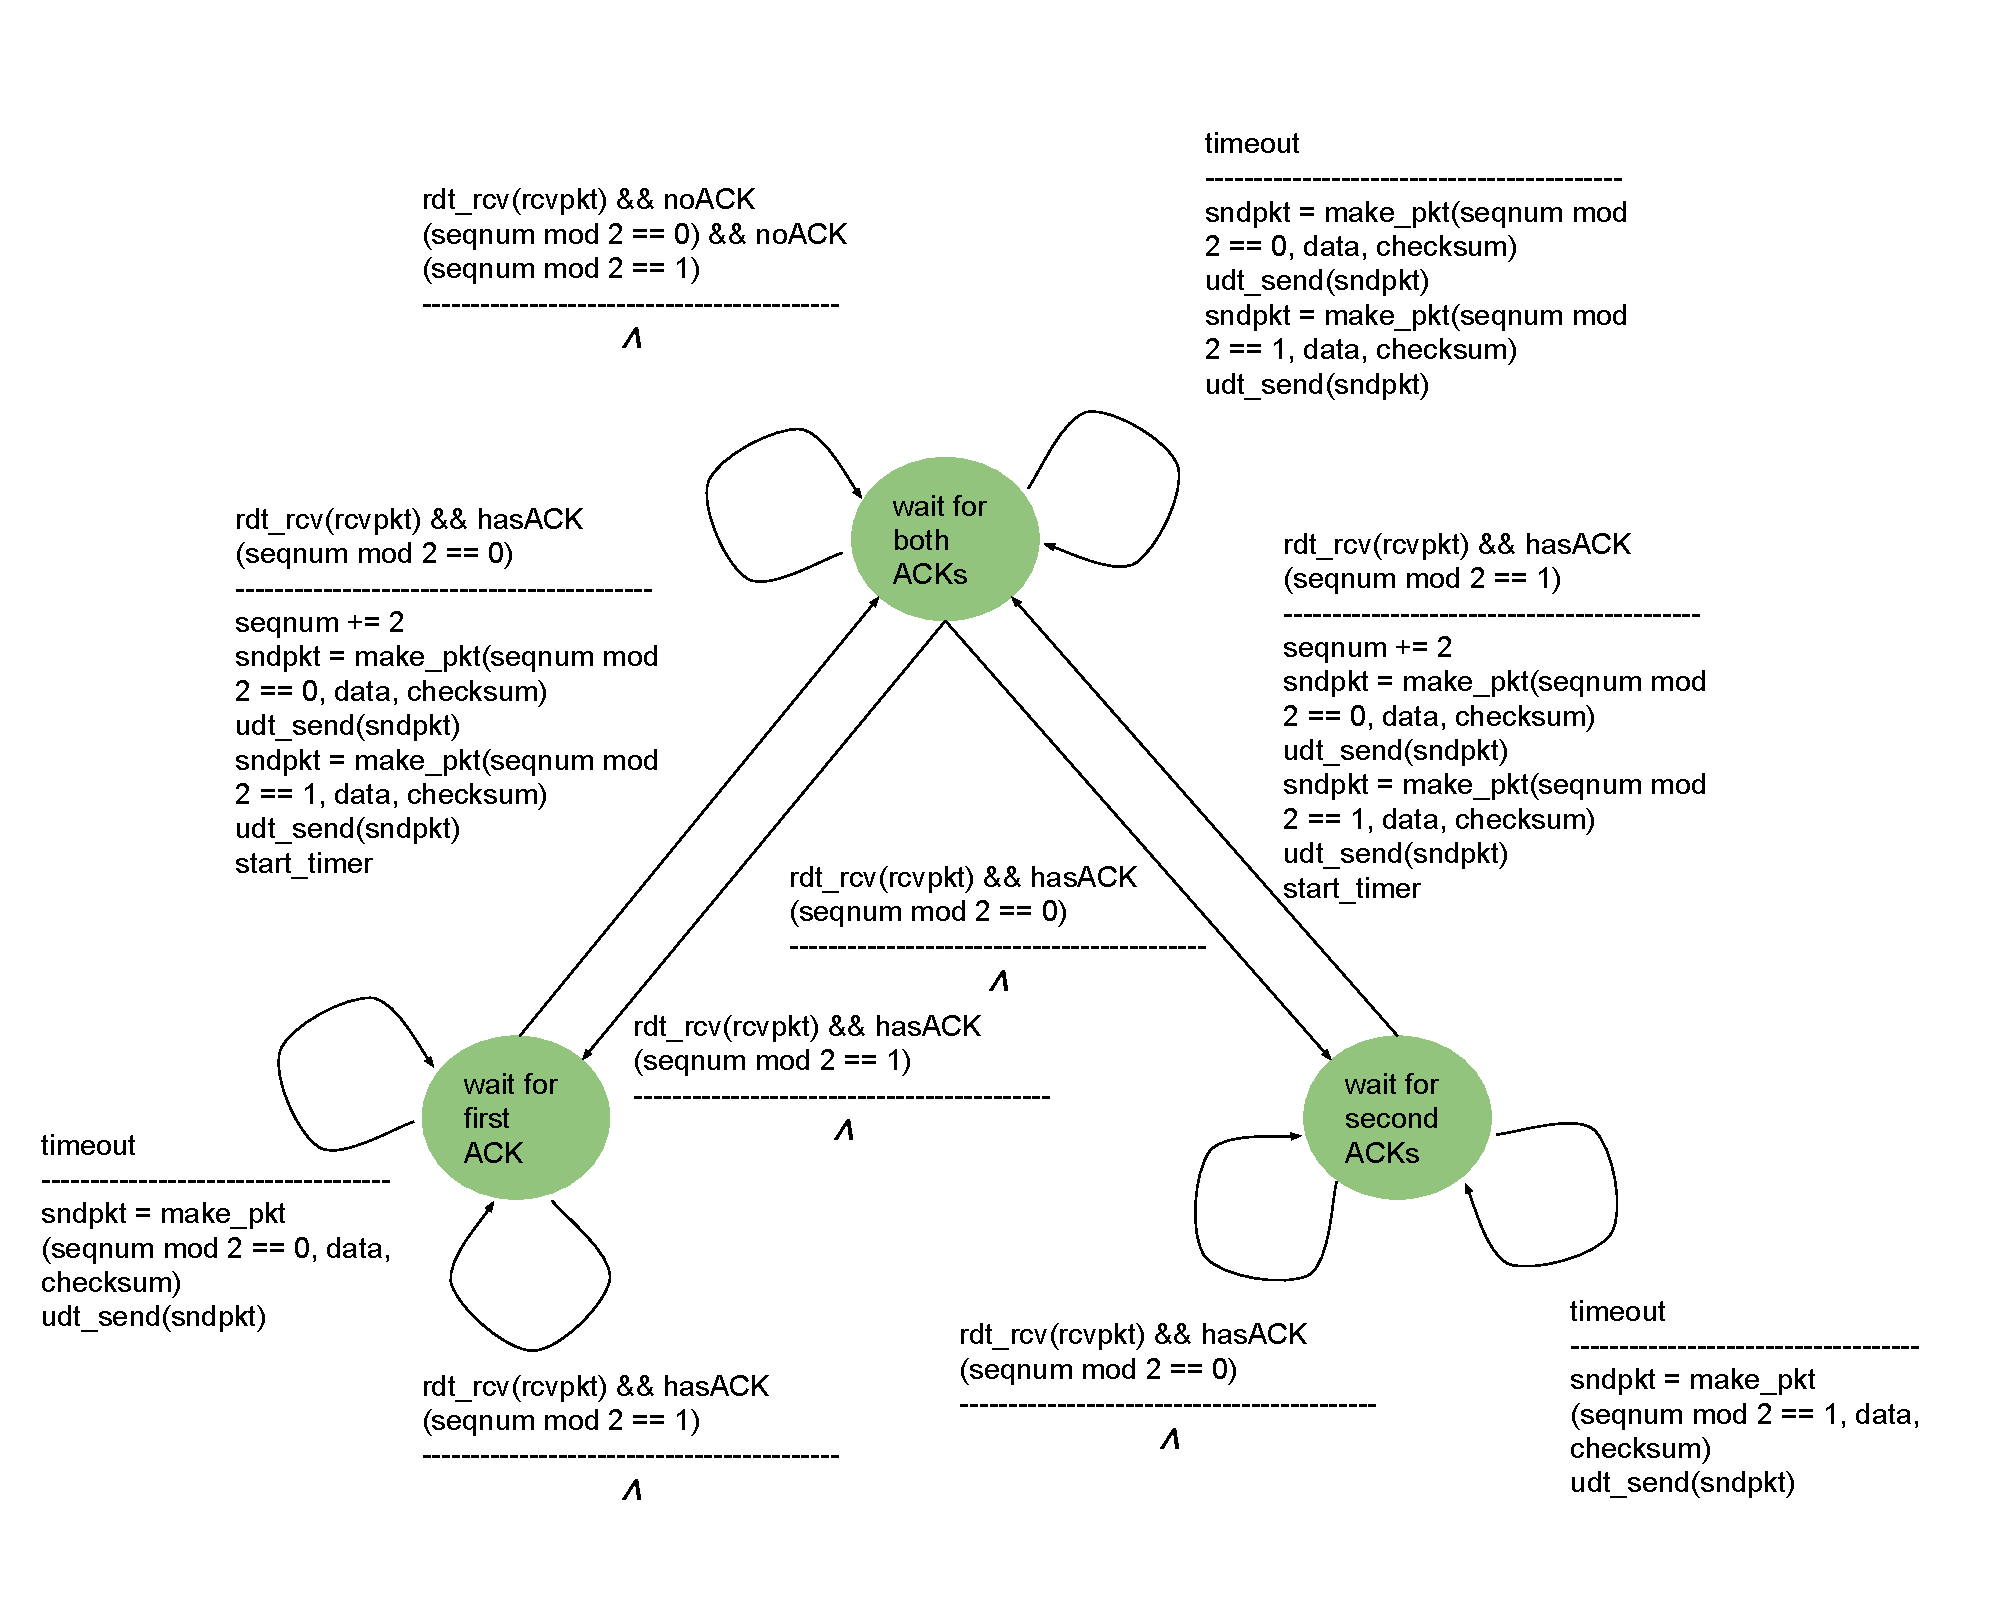
\includegraphics[width=\textwidth]{images/P18-sender.pdf}
    \caption{Sender FSM}
    \label{fig:p18-s}
\end{figure}
\begin{figure}[!ht]
    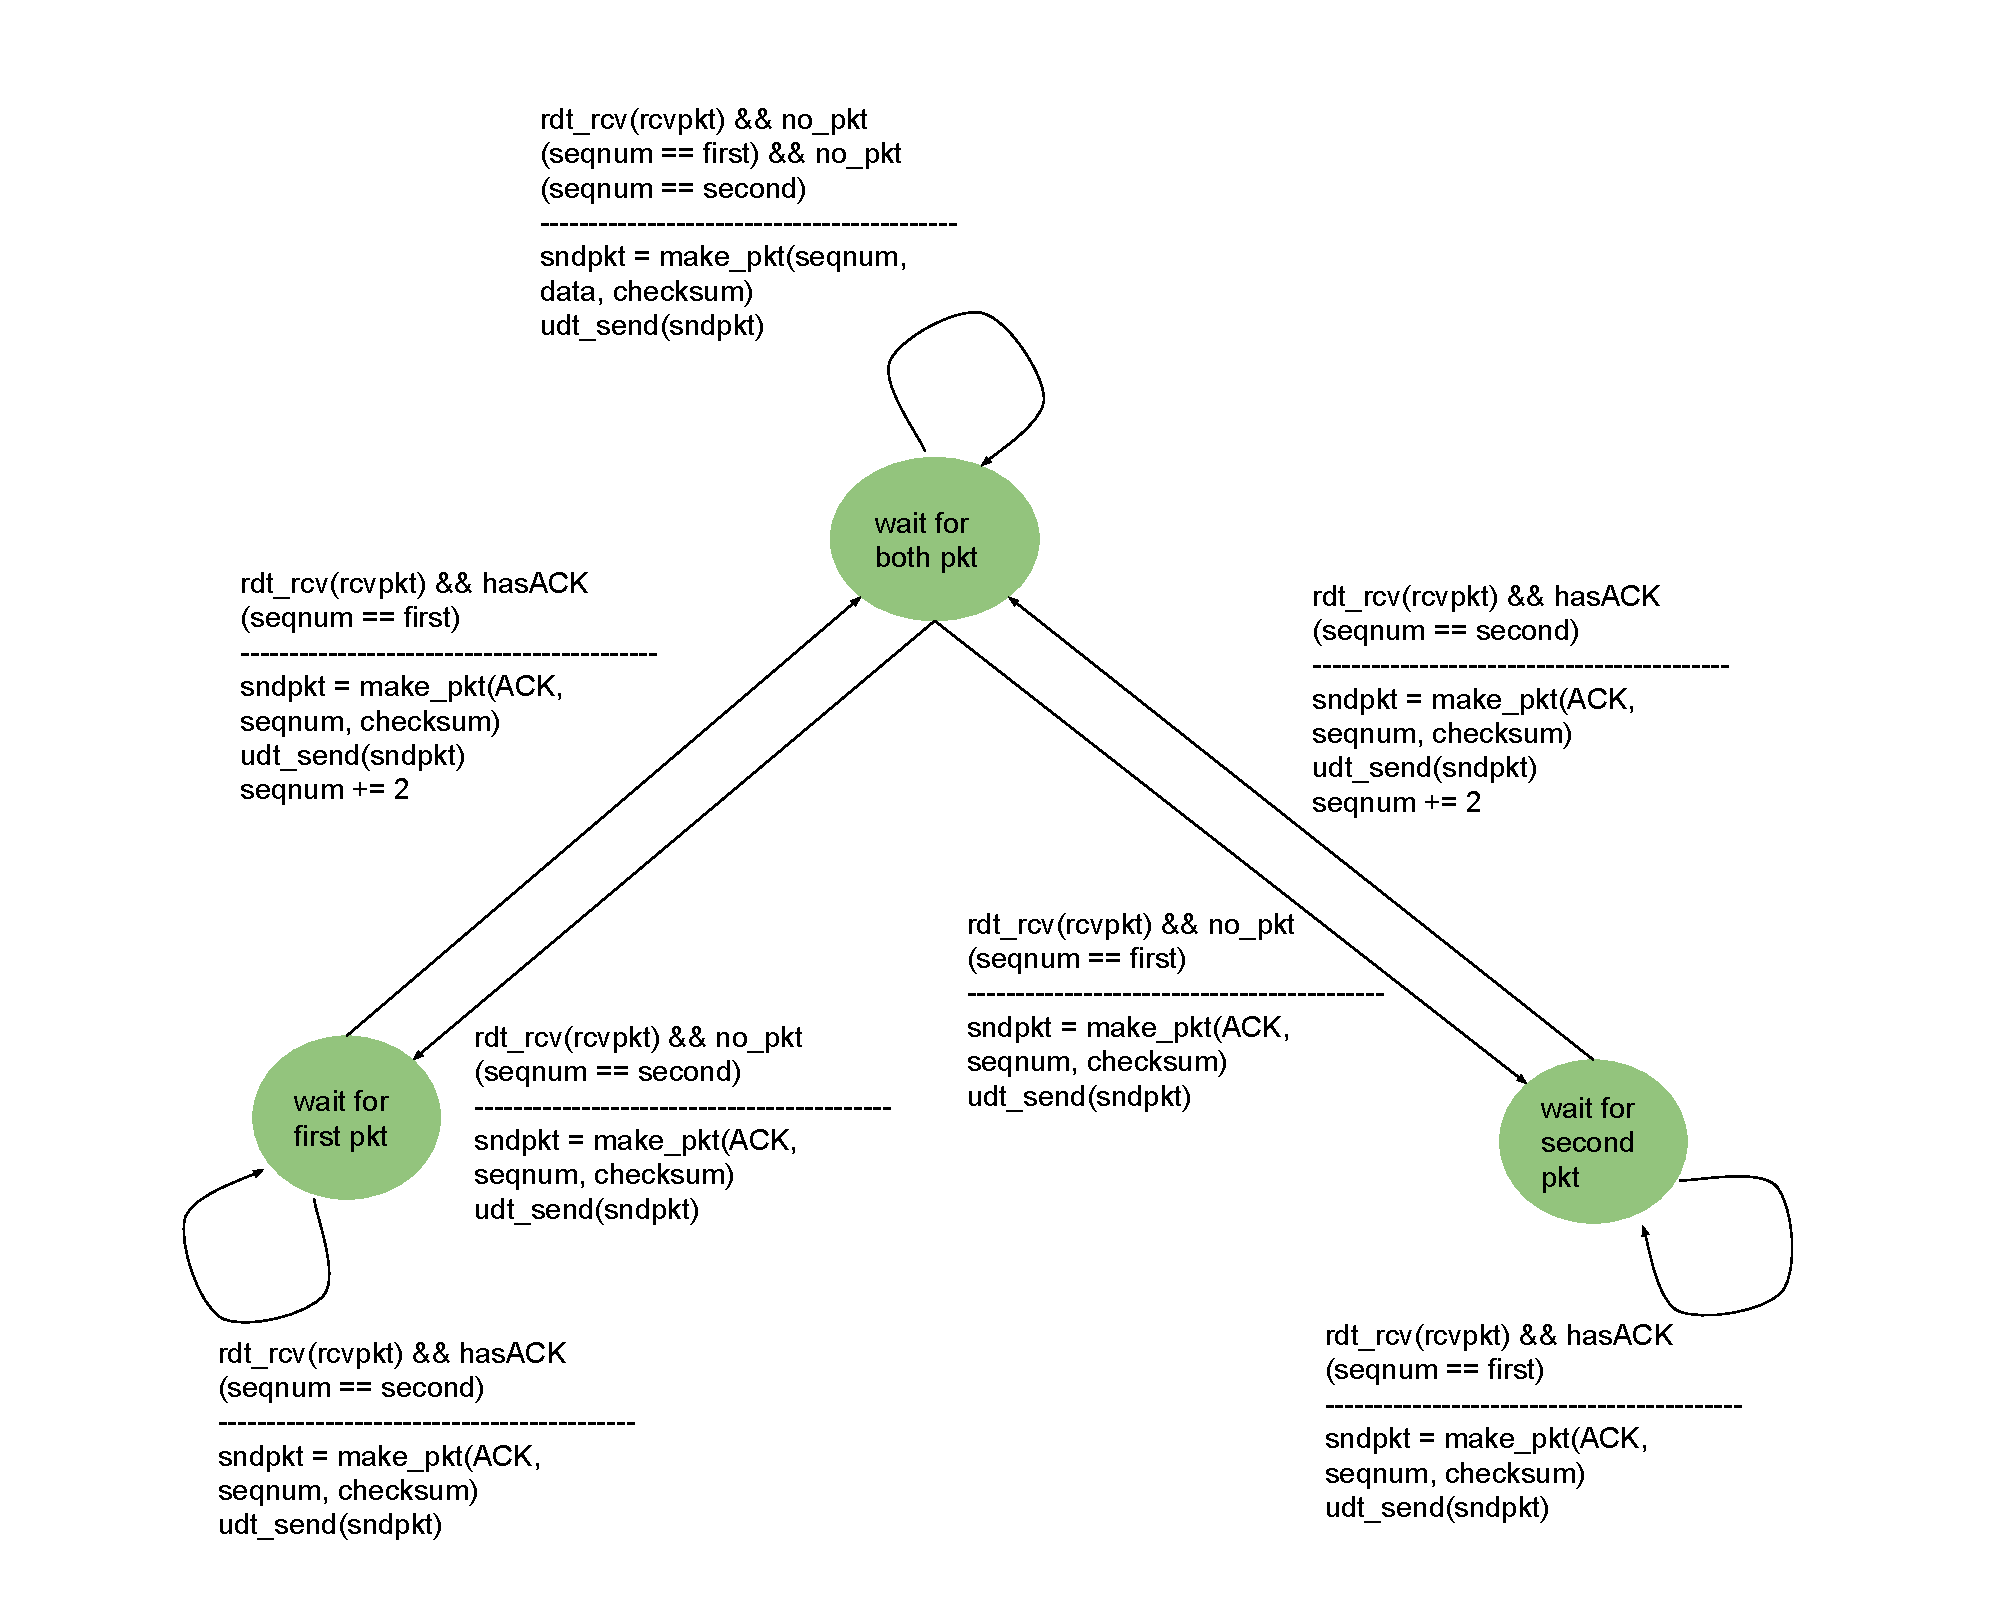
\includegraphics[width=\textwidth]{images/P18-receiver.pdf}
    \caption{Receiver FSM}
    \label{fig:p18-r}
\end{figure}
As an example of explaining how this protocol works, suppose sender sends (D0, D1).
D0 gets lost and D1 is successfully delivered. Once the receiver receives D1, it ACKs D1 with ACK1.
After sender receives ACK1, it stays in the state that waits for ACK0. But since D0 is lost, there will be no ACK0 until timeout occurs. Then sender resends D0. Receiver receives D0 this time and sends back ACK0. Sender gets ACK0 and goes back to the initial state to send a new pair (D2, D3).



%----------------------------------------------------------------------------------------
%	PROBLEM 22
%----------------------------------------------------------------------------------------

\section*{Problem 22}
\textbf{(a). }
Assume all the previous k-1 ACKs are successfully received by the sender, the sender base is now at
k. So the window looks like [k, k+3]. \\
Also, there is another possibility that ACK for k-1 is lost. So the sender base is at k-1, and the window looks like [k-1, k+2]. Similarly, there could be multiple ACKs lost up to k-1. Thus the sender window can also be [k-2, k+1], [k-3, k] and [k-4, k-1]. \\

\textbf{(b).}
Since the receiver is expecting k, it means it has already received k-1. And the window size is 4, so the oldest unacknowledged packet can be k-4. Thus, the propagating ACKs could have value k-4, k-3, k-2, k-1.
\\


%----------------------------------------------------------------------------------------
%	PROBLEM 23
%----------------------------------------------------------------------------------------

\section*{Problem 23}
By looking at Figure 3.27, we see that the receiver cannot tell whether packet 0 is a new one or a retransmitted one because the sender has the old packet 0 is its window and the receiver has the new packet 0 in its window. They are overlapped to be confusing. \\
To solve this problem, assume the receiver has window [k, k+w-1] where w is the window size. In the worst case discussed in problem 22, the propagating ACK could be k-w to k-1. If $k-w = k+w-1$ in the modulo k arithmetic, and unfortunately it is missing, then the receiver will be confused by the retransmitted packet k-w. Thus, k-w cannot overlap k+w-1. In other words, the window size should be at most half of the sequence number space.
\\



\end{document}
